% Optional analysis insert, compiled from the manuscript main/ directory.
\begin{figure}[htbp]
  \centering
  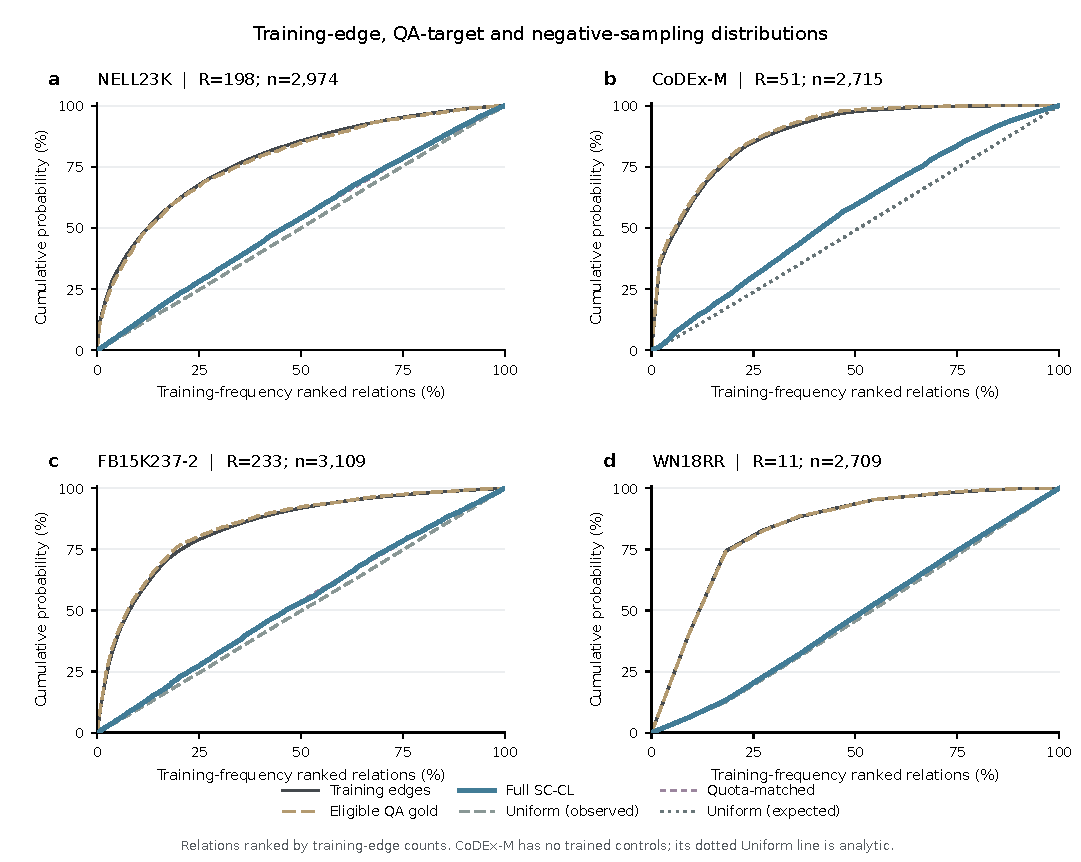
\includegraphics[width=\linewidth]{figures/sampling_distribution_seed2026/fig01_cumulative_four_datasets.pdf}
  \caption{四数据集的训练图关系质量、合格训练QA目标及冻结负候选累积分布。横轴在每个数据集内按训练边频次从高到低固定排序，纵轴为对应分布的累积概率；$R$为训练关系标签数，$n$为Full候选库覆盖的训练问题数。所有负库为seed2026、每题九个互异关系，不含gold。CoDEx-M没有已训练Uniform或配额控制，其均匀参考为各题合法池内均匀分布的解析期望。FB原始237个关系ID经既有文本映射对应233个训练标签；WN保留55条历史训练实体对核验缺口。曲线接近不等于预测等效或已确立机制。}
  \label{fig:sampling-marginals}
\end{figure}

\begin{figure}[htbp]
  \centering
  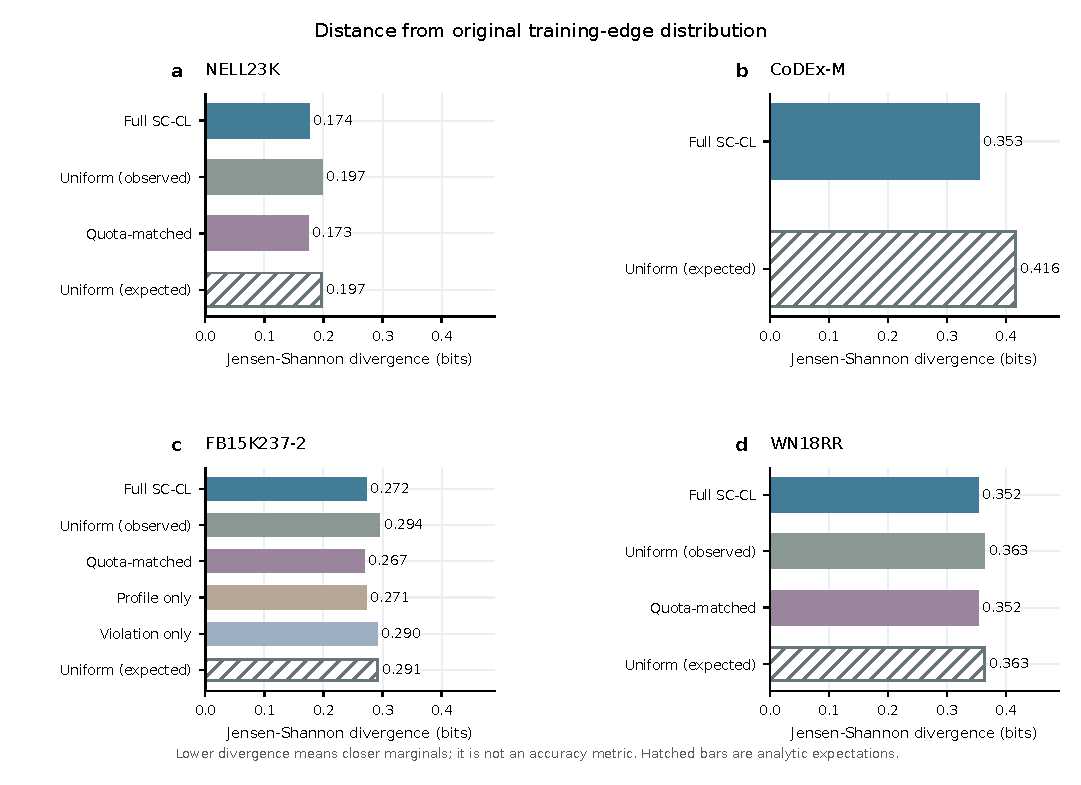
\includegraphics[width=\linewidth]{figures/sampling_distribution_seed2026/fig02_distribution_distance.pdf}
  \caption{冻结负候选分布到原始训练图关系边分布的Jensen--Shannon散度（base 2，范围$[0,1]$，越低表示边缘分布越接近）。Full分别为NELL 0.1743、CoDEx-M 0.3533、FB 0.2715、WN 0.3516；同题Uniform实测值为0.1970、未运行、0.2941和0.3628，CoDEx-M解析均匀参考为0.4157。斜线柱均为合法池解析期望，不是新增训练结果。所有结果描述一次冻结候选库，不提供跨种子误差条；较低散度不代表更高准确率。}
  \label{fig:sampling-divergence}
\end{figure}
